\chapter{Introduction}\label{ch:intro}

The \emph{IT-Security Awareness Penetration Testing Environment} (\ape)\cite{itsape} is a tool to analyse the awareness of a computer's user regarding IT-security. It measures the user's response to certain deployed \emph{artifacts} which differ from the user's familiar environment. Most of them are similar to real-world attack scenarios or share certain principles with them.

There are multiple aspects to the user's response, one of them being the reaction speed. For measuring the reaction speed one must determine the point in time from which on it is possible for the user to interact with the artifact. As \ape~is a tool for the Microsoft Windows operating systems (which focus on a graphical user interface, a \emph{GUI}), a user is able interact with an artifact as soon as he or she can visually perceive it on the screen, or in Windows terms: on the \emph{desktop}.

The process of finding this point in time can not be done reliably by observing the currently running processes or even meta information about it. Only the visual information of the current desktop is useful in this case: An extra feature or tool was needed to perform an image detection algorithm on the current screen and decide whether the visual cues of the currently deployed artifact are present on the user's desktop.

The most important measure for this tool would be the \emph{sensitivity}, describing the probability of successful detection of artifacts when they are actually present (\emph{true positives}). This term will be called \emph{detection rate} in the rest of this work and should ideally be at $100\%$. The counter-measure for this is the \emph{specificity} which describes the rate of \emph{true negatives}. A second, equally important measure is the resource consumption for execution, especially the execution time. As the detection rate is an obvious measure for such a tool, the execution time and resources are almost equally important to not disrupt the user's experience or distort the reaction analysis by \ape. The limitation on the resources is given by the environment that \ape~is mainly used in: low-tier office hardware.

The work at hand describes the design considerations and implementation details of such a tool, called \emph{\vad} (\emph{\vd}), and presents the results of an evaluation given the previously proposed measures. For this, chapter \ref{ch:rel-work} outlines some related publications and the differences to our approach. In chapter \ref{ch:methods}, the software design and technical details of the \vd~are explained. The evaluation setup for the given measures and the results can then be found in chapter \ref{ch:results}, followed by a conclusion in chapter \ref{ch:conclusion}.

As \ape~is designed for computers running \emph{Windows 7} in the 32-bit version, the \vd~was built for this operating system specifically but can run on newer Windows versions as well. Written in C\#, it uses Microsoft's \emph{.NET framework} in version 4.7.2 \cite{dotnet4_7_2} and the \emph{OpenCV}-wrapper \emph{Emgu CV} in version 3.4.3 \cite{emgucv}.

\chapter{Related Work}\label{ch:rel-work}

For evaluation of UI patterns Bakaev et al. \cite{ref_web-uis} use image recognition functions to analyse a website's screenshot and produce a machine-readable representation of it. A grayscale version of the screenshot is used for rectangle detection, text sections are identified and recognized, before detecting special UI element types using a trained feature extractor. The results are then used to analyse composite structures and output a textual representation of the website. While the task seems similar to the one presented in this report, the proposed analysis has different goals and does not suit the requirements for the \vd: The full classification of the screenshot before identifying possible candidates for artifacts would imply a high demand on resources and is not a necessary step. Since those candidates would then be compared to reference images of artifacts, one can skip the classification steps and use an image feature detector on the screenshots directly.

Aradhye et al. \cite{ref_spam-mails} present a way to classify image-based e-mails as spam using image analysis. Their approach features a way to analyse complex images without resorting to OCR: First, text regions are extracted by performing connectivity analysis on thresholded intensities of the grayscale image. With these regions identified, they categorize the image based on certain features which are then used to train \emph{Support Vector Machines} (\emph{SVMs}) to detect different mail classes. The key advantage of this way to classify images is that the spam images have distinct features to distinguish them from other images in mails. On one hand the \ape~artifact database is diverse and training SVMs for every artifact type would be demanding. On the other hand it is not easy to distinguish the more advanced \ape~artifacts from other applications by a rigidly defined feature set, because most of the artifacts \ape~employs try to imitate a usual application.

The goal of automated quality assurance lead Mozgovoy et al. \cite{qa_image-rec} to the usage of image recognition on GUIs. They identified a problem for conventional GUI-testing suites for games with non-standard GUI and other elements. Their solution decides against exact bitmap matching, as the elements could be transformed, and instead match them approximately against a template. Since their approach is unable to find scaled matches, they first scale the reference to the observed image and then match them in total. Here, the main difference to the task at hand lies in the references to match against: In their case the matched output should have limited variation compared to the references so that they are able to match the whole screenshot onto the scaled reference. This is not applicable for the use cases in \ape, as the artifacts are usually present in only a part of the whole screenshot. Since the rest of the screenshot is subject to high variation, building an adequate reference image collection for whole screens is highly infeasible.

Since none of the related work matches the goals for the \vad, a new tool had to be implemented.

\chapter{Methods}\label{ch:methods}

This chapter begins with a description of the general software design, including a brief requirement analysis and the resulting decisions regarding the implementation. The second part introduces the technical backgrounds and algorithms used, and especially explains the choice of the image recognition algorithms and their parameters.

\section{Software Design}\label{sec:software-design}

The client of \ape~that gathers the user's reaction to the deployed artifacts runs on a PCs as a Windows service. Instead of implementing the \vad~as an additional feature of the \ape~service it is implemented as an external tool. This is to keep a modular approach in which software parts can easily be exchanged, and secondly to be able to give the individual processes an independent priority for execution, thus guaranteeing enough resources for the execution of the \ape~service.

The main reason the \vd~was designed to run on the same machines as the \ape~service instead of e.g. a server infrastructure with better hardware or other external hardware was the user's privacy:  As \ape~aims to collect the data anonymously or pseudonymously, transactions of highly sensitive data (such as screenshots of the current desktop) would contradict this goal.

The information on artifact types to detect are provided by a \emph{recipes repository} on the same computer containing reference images of the artifacts to be deployed. Furthermore, the \vd~only has to look for visual cues of a single artifact type per run, as the \ape~service will call it with information on the currently deployed artifact type and the path to a screenshot to analyse.

\subsection{Requirement analysis}

To implement the \vd, the following main requirements were identified:

\begin{enumerate}
	\item \label{itm:req-detection} Robust and high detection rate for visual cues of artifact in screenshots of a Windows desktop.
	\item \label{itm:req-lowruntime} Low runtime of at most few seconds on low-tier office hardware.
\end{enumerate}

These requirements reflect the measures given for this task in the first chapter. The \ref{itm:req-detection} requirement mainly has influence on the choice of image recognition algorithms, while the \ref{itm:req-lowruntime} contradicts the use of a very resource-heavy algorithm (which would provide better results, generally speaking) and has influence on the parameters of the used algorithm. This could lead to a trade-off between the \ref{itm:req-detection} and the \ref{itm:req-lowruntime} requirement which is referred to in section \ref{sec:tech-bg}.

Further analysis of the nature of \ape~and refinement of the main requirements lead to the following secondary requirements:

\begin{enumerate}\setcounter{enumi}{2}
	\item \label{itm:req-nocuda} No usage of parallel computing on the graphics card (e.g. with the CUDA Toolkit\cite{cuda}), CPU only.
	\item \label{itm:req-win7console} Windows 7 console program (32-bit).
\end{enumerate}

The \ref{itm:req-nocuda} requirement is a specification of the \ref{itm:req-lowruntime}, as low-tier office computers usually don't include a CUDA-enabled graphics card or a non-integrated graphics card at all. This requirement results in better versatility of the tool, but comes at cost of a higher runtime.

Given the deployment area for \ape~in the present and near future, the \ref{itm:req-win7console} requirement is due to the environment \ape~is mainly run in. This is also important for the nature of the visual cues of artifacts which mainly are those of standard Windows GUI objects.

\subsection{Implementation decisions}

It was initially decided to use an existing library for image recognition rather than implementing the algorithms anew. The choice for an image recognition library fell to OpenCV, as it is licensed as \emph{Open Source} under the BSD license and arguably the most maintained and popular of such libraries with almost 20 million downloads \cite{opencv_downloads}. Other libraries for similar tasks exist, but they either focus more on machine learning like \emph{Google's Tensorflow} \cite{tensorflow}, are web-based APIs (mostly non-free) like \emph{Google's Vision API} \cite{vision_api} or \emph{Amazon Rekognition} \cite{rekognition}, or are not well maintained, such as \emph{VLFeat} \cite{vlfeat}.

Because the runtime performance is so important for this tool, it was not suitable to implement the program using an interpreted programming language. The usage of OpenCV limits the available compiled languages to C, C++ or Java, and using the wrapper Emgu CV also allows to use C\#.

The advantage of C\# is the possibility to use Microsoft's \emph{.NET Framework} \cite{dotnet4_7_2}. It allows to efficiently implement Windows 7 programs while the latest \emph{redistributable packages} of .NET needed for executing .NET programs are available per default (given the system is up-to-date). Furthermore, the speed differences between the execution of .NET's intermediate language in their \emph{Just-in-Time} compiler are nowadays insignificant to programs written in e.g. native C++. Therefore the \vd~is written in C\# using .NET 4.7.2 and OpenCV 3.4.3 via the Emgu CV wrapper.

During evaluation it was noticed that the used post-processing function by Emgu CV lead to erroneous results and it was decided to code an own implementation of it as a replacement (see subsection \ref{sec:tech-bg:subsec:outlier-rejection} for details).

Furthermore, a Windows installer setup was composed to allow easy deployment of the \vd~after compilation.

\section{Technical backgrounds}\label{sec:tech-bg}

The process of image recognition in the \vd~expects two input images per run, one model image and one observed image, and tries to recognize the model in the observed image. The model image is a reference image of the artifact type to detect and the observed image is a screenshot provided to the program at execution time. Since the given artifact type may have multiple reference images for several characteristics, this process might be performed as many times as there are reference images, but exits as soon as a match between a reference and the screenshot was found. This is especially important for the performance, as the order of the artifact's reference images are directly affecting the runtime (see chapter \ref{ch:results}).

The goal of the recognition process is to find a valid transformation matrix to the model's features for the largest possible subset of the observed image's features. If such a matrix can not be found for a subset of certain size, it is decided that no match exists. There are three major steps involved in the image recognition process: \emph{Feature detection and description}, \emph{feature matching} and \emph{outlier rejection}, while the last step includes finding a transformation matrix.

The first step yields a set of features extracted from the observed image. This is also done for all of the model images, but their feature set could be fetched from a cache if extracted in a previous run, which effects the performance (see chapter \ref{ch:results}). The features are represented as feature descriptors which are then matched with the model's descriptors, resulting in a set of candidates for features found in both images. These are then post-processed during outlier rejection to find a transformation matrix from one feature subset to the other while matching the most candidates. If there is such a matrix fitting to a certain percentage of the candidates (see subsection \ref{sec:tech-bg:subsec:outlier-rejection}) the \vd~will return the successful detection of the artifact (return value $0$). Otherwise, it will return that no match was found (return value $1$).

\begin{figure}[h!]
	\centering
	\includegraphics[scale=0.23]{fig/example-debug-output.jpg}
	\caption{Example debug output of the \vd~when finding a match. On the left side is the observed image, on the right the model. Yellow circles show match candidates, green lines connect actual matched feature points. A red rectangle is drawn around the recognized area.}\label{fig:example-debug-output}
\end{figure}

In figure \ref{fig:example-debug-output} an example of debug output for a successful match can be found with the observed screenshot drawn in the left half and the reference screenshot in the right. There are more match candidates marked than are actually used as match, which shows the results of the outlier rejection step. The transformation matrix has been used to draw the rectangle around the area where the artifact has been successfully recognized. Since the artifact's window partly lays outside of the screenshots boundaries, the red rectangle appears cut off as well.

The retrieval of the transformation matrix can take advantage of the special properties of the deployed artifact's being mostly standard GUI elements: There are only few possible transformations for Windows GUI objects: First, they can be translated versions of the artifact's reference images. In this case, the transformation matrix is easy to find and this transformation is the most common one. Secondly the GUI objects can be scaled in a sometimes complex manner, e.g. by shifting sub-parts of the object to different locations and changing the aspect ratio between feature points. The combination of both transformation is the third possibility. It is hard to impossible to find a single transformation matrix for the last two of the mentioned transformations, but sometimes sub-parts of the image can be recognized more easily. For this reason the \vd~in the current implementation mainly focusses on detecting the first kind of transformation reliably and leaves the improvements in the recognition of the complex transformation for future work.

The following sections will describe the choice of algorithms for each step and their configuration details.

\subsection{Feature detection with ORB}\label{sec:tech-bg:subsec:feature-detection}

The set of available algorithms for feature detection were provided by the implementations in Emgu CV, respectively OpenCV. From those, as shown in secondary literature such as Tareen et al. \cite{orb_comparison}, ORB configured to find a limited amount of features provides the best combination of resource usage and result quality compared to the other three algorithms.

The ORB (\emph{Oriented FAST and Rotated BRIEF}) keypoint detector and descriptor is a ``very fast binary descriptor based on BRIEF [...], which is rotation invariant and resistant to noise'' \cite[p.~1]{orb}. It is specifically designed for real-time systems and low computing power, thus being faster than most of the other currently available methods \cite{orb, orb_comparison}. As the name states, it combines an enhanced version of the \emph{FAST} \cite{fast} keypoint detector with \emph{rotation-aware BRIEF} (\emph{rBRIEF}) \cite{brief} descriptors. \cite{orb, fast, brief}

The FAST (\emph{Features from Accelerated Segment Test}) detector \cite{fast} is a corner detector designed for real-time applications, working on pixel-regions with fixed radius. The ORB detector utilizes an extended version of the FAST detector with a patch radius of $9$. This radius has proven to yield the most reliable results, where reliability is defined as the rate of detecting the same corners in multiple views of an object. This reliabilty is proven in the evaluation results in section \ref{sec:eval-results:subsec:dect} as well. \cite{fast, orb}

The extended FAST detector employed in ORB is used to detect corners on a pyramid scheme for scale variants \cite{scale_pyramids} of the image. At instantiation of Emgu CV's implementation of ORB one can adjust the scale factor and number of levels for those pyramids. For the \vd~the preconfigured scale factor $1.2$ with $8$ levels was used. Since the \vd~currently responds poorly to scaled versions of the artifact's reference images these settings could be adjusted in future versions (see chapter \ref{ch:results}).

After detection, a \emph{Harris corner filter} \cite{harris_corner} for rejecting edges is applied to the top keypoints with the strongest FAST responses \cite{orb}. The feature detection process in the Emgu CV implementation of ORB is done until a configured amount of features are found (if possible), the preconfigured amount in Emgu CV being $500$ features. This amount was doubled for the \vd~to extract up to $1000$ features per image, as a higher value allows for better differentiation between the reference images. An even higher amount of features affects the execution time negatively while not resulting in better matches for the provided reference screenshots.

There are more configuration parameters available for ORB, but the preconfigured values were found to be sufficient for this task.

\subsection{Descriptor matching}\label{sec:tech-bg:subsec:descriptor-matching}

The matching step tries to find one or more descriptor of the model image's keypoints (called the \emph{training set}), for each of the observed image's keypoints (called the \emph{query descriptors}). For feature matching, there are only two possibilities implemented in Emgu CV: Brute-force matching and \emph{FLANN} (\emph{Fast Library for Approximate Nearest Neighbor}) \cite{flann} based matching. There are different matching algorithms implemented for both of them such as the \emph{k-nearest-neighbor} algorithm (\emph{k-NN}).

FLANN based \emph{k}-NN-matching performs best for large datasets with high dimensionality, but is less likely to find all possible candidates for matches \cite{flann}. The trade-off between the focus on speed and accuracy mentioned in section \ref{sec:software-design} lead to the choice of FLANN based k-NN-matching for better performance. For the \vd~$k$ was set to $2$, so that for each query descriptor, the $2$ nearest-neighbor descriptors from the training set are returned -- if possible. The choice of $k$ allows to apply several post-processing filters (see subsection \ref{sec:tech-bg:subsec:outlier-rejection}) which reduce the overall recognition time.

\subsection{Outlier rejection}\label{sec:tech-bg:subsec:outlier-rejection}

The best $k$ matches for each query descriptor are filtered in several steps before trying to find a transformation matrix using the \emph{Random Sample Consensus} (\emph{RANSAC}) \cite{ransac} algorithm. These filtering steps try to exclude as many match candidates as possible from the given query descriptor set so that the process can be stopped early if there are not enough match candidates left. The match candidates that do not match the correct features are called \emph{outliers}, while the ones that do are called \emph{inliers}.

\begin{figure}[h!]
	\centering
	\includegraphics[scale=0.3]{fig/distance_threshold_orb.png}
	\caption{Analysis of the relation between descriptor distance and frequency of the match being an inlier or outlier, dotted for outliers and solid for inliers \cite[p.~4]{orb}.}\label{fig:dist-thresh}
\end{figure}

Since the 2-NN-matching can yield less than two matches for some query descriptors, only those descriptors that have two matches are taken into account for the next steps. The first test is the distance threshold filter proposed in the original ORB publication \cite{orb}. Their analysis of the distance of a match compared to the probability of it being an inlier or outlier showed, that above a certain distance a match candidate is unlikely to be an inlier. For the \vd~a threshold of $80$ was chosen, as it is the approximate turning point of the probability for the candidate being an outlier rather than an inlier when using rBRIEF descriptors (see figure \ref{fig:dist-thresh}). The second filter is an implementation of \emph{Lowe's ratio test} \cite{lowes_ratio} with the recommended distance ratio of $0.7$ between the first and the second match's distance. After these steps, two functions provided by OpenCV/Emgu CV are used to eliminate duplicates and to rule out candidates that do not have the size and orientation of the majority of match candidates.

Between and after those filtering steps the \vd~determines the current count of match candidates and checks if there are still enough for a successful match. They are compared to a fixed threshold parameter $min_{\text{matches}}$ of $25$ divided by the ratio of the observed and model images' areas. This parameter $min_{\text{matches}}$ has been found empirically to be the best trade-off between a suitably high detection rate given the currently implemented artifact types in \ape~and still skipping most of the matching process early if a match is improbable. The ratio of the image's areas allow model images to be found that have a small image size comparison to the observed image. This is a necessary factor, as the density of the feature descriptors per image area becomes more sparse if the image size becomes larger.

At the last step of image recognition, if there are enough candidates left, an own implementation of RANSAC is performed. Two match candidates are randomly sampled and are used to calculate translation and scaling factors for a hypothetical transformation matrix. This hypothesis is then tested on all match candidates allowing a transformation error of an $11x11$ pixel patch due to the inaccuracy of floating point arithmetic for C\#. If a certain percentage of candidates support it, given by the confidence parameter, a match was found.

The iteration count of RANSAC was set to $1000$ iterations. This is derived from the square of$min_{\text{matches}}$ adjusted upward to the next power of ten to allow for an error margin, respectively a high area ratio factor. In the best case scenario this iteration count allows the minimum of needed match candidates to be combined. The confidence factor was set to 85\% via empirical analysis, meaning that only 15\% of the remaining candidates may be outliers of the hypothetical matrix.

The calculation of the translation and scaling factors in this part is influenced by the observation of possible transformations for GUI elements. In the current implementation a high detection rate despite arbitrary translation of the Windows GUI elements is the main focus while detecting other, more complex transformations is a secondary concern.

\chapter{Results}\label{ch:results}

The \emph{Artifact Detector} was evaluated in an environment that should closely resemble the real-world application domain of \ape. In section \ref{sec:eval-env} the evaluation setup is explained in detail.

There are two main focus points for the evaluation, reflecting the measures given in chapter \ref{ch:intro}: First, a qualitative analysis of the detection rate for 25 randomly chosen artifact types from the \ape~recipes repository is presented. Then a quantitative analysis of the used execution resources follows, using eight specially crafted artifact types to control as many factors as possible. The results for those two parts can be found in section \ref{sec:eval-env}.

The \ref{itm:req-lowruntime} requirement resulted in the implementation of a \emph{cache} for already processed data of artifact images from previous runs. This leads to drastic runtime improvements in consecutive runs of the same artifact type, but is opposed by another factor: As soon as the size of the cache increases, the duration of loading and decoding increases as well. Even for a small count of artifact types of three or four types the loading time becomes larger than the time saved by caching. Therefore, the cache was discarded and not used during evaluation. Its concept could still be continued in future work (see chapter \ref{ch:conclusion}).

\section{Evaluation setup}\label{sec:eval-env}

For the evaluation Windows 7 was setup on a virtual machine using Oracle VM VirtualBox\cite{virtualbox}. This allowed an easy setup and quick configuration of the available hardware. All official Windows 7 updates were installed on this VM up to those available at the 25th of March 2019. No additional software was installed other than VirtualBox's \emph{Guest Additions}, which are necessary to share data between the host and the virtual machine.

The virtual machine was run with 2GB of RAM available and one core of an Intel Core i5-6600K CPU (3,50 GHz) set to a 40\% execution cap, resulting in a single virtual CPU at a speed of 1.4 GHz. These hardware settings were thought to approximate low-tier office hardware sufficiently enough to allow conclusions for the real-world application domain of \ape.

After installing the \vd~in the virtual machine using the installer provided, a Batch-script runs the executable multiple times using data supplied in shared folders by the host system. The supplied data was chosen such that it fitted the respective evaluation focus.

\section{Evaluation results}\label{sec:eval-results}

The evaluation results presented in this section prove the successful implementation of the \vd~regarding the detection rate and resource usage, but hint to several aspects to improve in future work. This is especially true when it comes to the length of the execution time.

Given the test-setup described in subsection \ref{sec:eval-results:subsec:dect} the detection rate was found to be at about $90\%$ in total. While the execution time for artifact types with few or conveniently ordered reference images has a median of less than 500ms per run, the amount and order of reference images seem to influence the execution time in a linear way. For each additional image that has to be loaded and processed, the \vd~needs an extra 150ms to 250ms to compute a result (see subsection \ref{sec:eval-results:subsec:res}). This can lead to execution times deemed too long for application in the \ape~environment and thus needs improvement.

\begin{figure}[h!]
	\subfigure[Results for artifacts A1 to A12.]{
		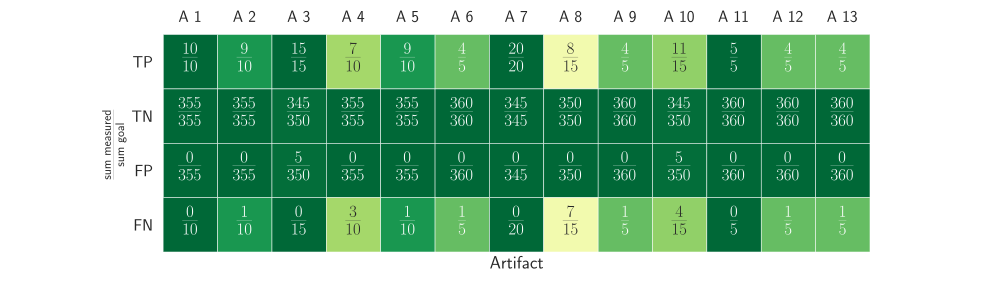
\includegraphics[scale=0.5]{fig/quality-confusion-matrix-p1.png}\label{fig:result-quality-p1}
		}\hfill\\
	\subfigure[Results for artifacts A13 to A24 and their totals.]{
		\includegraphics[scale=0.5]{fig/quality-confusion-matrix-p2.png}\label{fig:result-quality-p2}
		}\hfill\\
	\caption{Detection rate for all runs by artifacts A 1 to A 24 and their totals}\label{fig:result-quality-sum}
\end{figure}

\subsection{Detection rate}\label{sec:eval-results:subsec:dect}

For measuring the detection rate, 25 randomly chosen artifact types from \ape's original artifact library have been selected. They have been numbered A 1 to A 25 according to table \ref{tab:abbr_artifacts} in the appendix. Each of their reference images has been merged with a collection of five different Windows desktop screenshots to create a large set of testing screenshots. This merging is done programmatically and places the reference image at a random position on the desktop screenshot such that at least $90\%$ is still inside the images boundaries. In addition to the reference images, screenshots of objects that do not belong to any artifact type, but resemble common desktop applications have been processed in the same way. This leads to a total of 365 generated screenshots for the quantitative evaluation.

For the test run, the \vd~was executed with each of the 25 artifact types as targets on each of the 365 screenshots (9125 executions in total). The returned value has then be compared to whether the artifact type is actually present in the screenshot. The summed up measurements for each artifact type can be found in figure \ref{fig:result-quality-sum}, where the y-axis denotes the categories \emph{true positive} (TP), \emph{true negative} (TN), \emph{false positive} (FP) and \emph{false negative} (FP). Each cell shows the relation between the actual results (numerator) and the correct result (denominator). In the last column of subfigure \ref{fig:result-quality-p2}, the summed up results of all artifacts can be found. The cells are color coded in a spectrum from red at $0\%$ over yellow at $50\%$ to green at $100\%$ for TP and TN and vice-versa for FP and FN.

The results show that the sensitivity of the result is $>88\%$ for the summed up total, while the specificity is at $>99\%$. Although the sensitivity is above $50\%$ for all tests, some artifact types show a significantly lower sensitivity. This is especially prominent for A 4, A 8, A 10 and A 17, for which the \vd~has a detection rate between $53\%$ and $70\%$. This is most probably due to these types' reference images, which have very few distinct features even for human perception. Anomalies in the specificity are only found for A 4 and A 10, with each of them having five false positive matches. Cross-checking the screenshot collection showed that a highly similar reference picture was used for both artifact types, only differing in a small text region and resulting in five evaluation screenshots each. Those were then identified as a match by the opposite artifact type. In conclusion, both error sources can be depleted by choosing more distinct and feature-rich reference images for the artifact types.

A second test run under the same conditions showed the exact same detection rates for all executions, proving the robustness of ORB's extracted features.

For measuring the detection rate of scaled versions of the artifact types, a second collection of screenshots was generated containing stretched versions of the reference images. This resulted in a sensitivity below $50\%$, showing that the algorithm does not reliably detect such scaling. But since the artifacts would not be transformed in this way for real-world use-cases this result is not substantial for the assessment of the overall success.

\begin{figure}[h!]
	\centering
	\subfigure[Execution time for loading the searched artifact's reference images.]{
		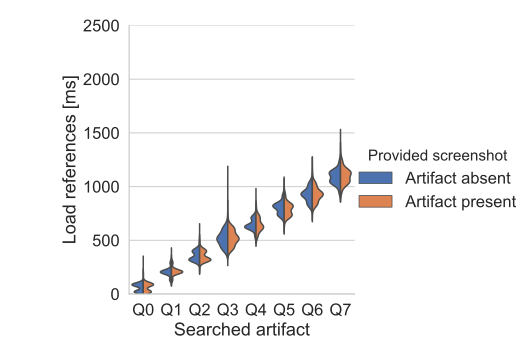
\includegraphics[scale=0.4]{fig/quantity-violin-load.png}\label{fig:result-quantity-load}
		}\qquad
	\subfigure[Execution time for extracting the observed screenshot's features.]{
		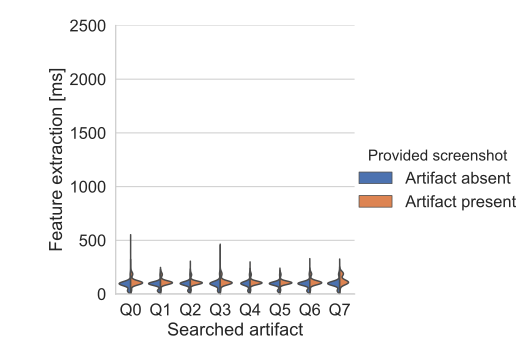
\includegraphics[scale=0.4]{fig/quantity-violin-feature_ext.png}\label{fig:result-quantity-feature_ext}
		}\\
	\subfigure[Execution time for matching the feature descriptors and finding a transformation matrix.]{
		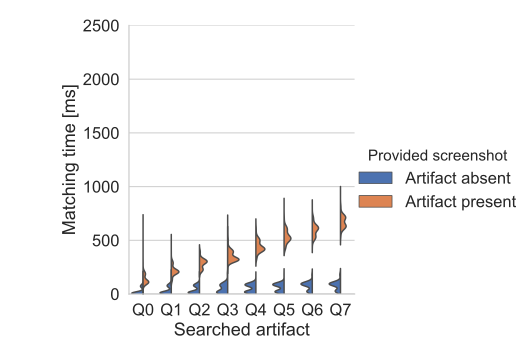
\includegraphics[scale=0.4]{fig/quantity-violin-matching.png}\label{fig:result-quantity-matching}
		}\qquad
	\subfigure[Execution time sum of all three image recognition parts.]{
		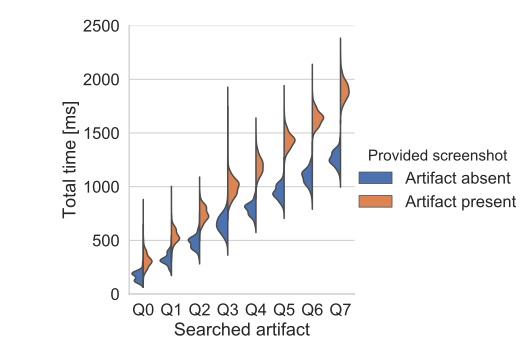
\includegraphics[scale=0.4]{fig/quantity-violin-total.png}\label{fig:result-quantity-total}
		}
	\caption{Execution times for artifacts Q0 to Q7}\label{fig:result-quantity}
\end{figure}

\subsection{Execution resources}\label{sec:eval-results:subsec:res}

A different setup was used for the quantitative analysis of the \vd: Eight new artifact types were constructed, named Q0 to Q7. If the artifact is actually present in the tested screenshot the artifact's index denotes at which position of their provided reference images the only matching image to the queried screenshot is located. The matching reference image is always the last reference image to test, so that Q0 has one reference image in total, Q1 has two etc. There are only two screenshots used for the tests, one with the artifact present ($s_ap$) and one without, the latter being an empty desktop screen ($s_aa$). The test is set up such that only the last step of outlier rejection is skipped if the artifact is present in the screenshots, namely the execution of RANSAC to recover a transformation matrix. This is achieved by choosing a non-matching reference image which has enough similarities to the matching one and allows to assess the influence on the runtime of the RANSAC implementation.

Each of the two screenshot gets queried 1000 times for each artifact type Q0 to Q7, resulting in $16000$ executions of the \vd~in total. The high count of repetitions is used to even out randomly occurring errors that have an influence on the execution time so that the sample is as representative for the execution time as possible. The results are depicted in figure \ref{fig:result-quantity} using a violin plot with a kernel density estimator of $0.5$.

The first plot in figure \ref{fig:result-quantity-load} shows the execution time in ms needed for loading all of the type's reference images and extracting their features. The increase of the duration dependent on the image count can be assumed to be linear given the implementation. This is an expected behaviour and matches the results of the second plot in figure \ref{fig:result-quantity-feature_ext} which is showing the duration of the same process for the observed screenshot. Since for all runs there is only one observed screenshot to extract features from, the time needed for this task is constant in a certain error margin. Both plots also show the independence of these steps from the actual absence or presence of an artifact.

Plot three in figure \ref{fig:result-quantity-matching} shows the duration of the last two step of the recognition process (from here: \emph{matching time}), namely feature matching and outlier rejection. One can see how the presence of the artifact in the image drastically increases the matching time. With only eight of such artifact types it is not possible to distinguish the type of increase depending on the reference count, but a linear increase is probable. The difference in execution time for $s_ap$ and $s_aa$ show, how the threshold checking of the match count prevents the execution of further filtering steps and thus saves execution time. It also shows a large influence by RANSAC on the execution time.

In figure \ref{fig:result-quantity-total} the sum of the previous three values is plotted. It shows that the image recognition process of the \vd~takes at least 100ms ($s_aa$) to 250ms ($s_ap$) and can take up to 2000ms or more, if there are multiple reference images in an inconvenient order. The plot also shows that there is a significant difference for $s_ap$ and $s_aa$ in execution time which is only due to the difference in matching time.

There are major outliers for the measured times of each step, being up to double to triple the time of the median. The reason for this is likely to be be a delay in access to the file storage if it occurs while loading and extracting the references or screenshot. For all steps it is also possible, that an increased CPU-usage by some other program decreased the resources available for the \vd, although such an execution was tried to be suppressed in the virtual machine.

Since the tests are run in a virtual machine, the built-in tools for VirtualBox have been used for measuring the resource consumptions at random points during the execution. The RAM usage of one of \vd's instances was between 30MB and 45MB consistently, while the CPU usage was at almost $100\%$ for all runs.

\chapter{Conclusion}\label{ch:conclusion}

The evaluation showed the importance of the quality of reference images for the detection rate, although for most types in the recipes repository the reference images were \emph{good enough} to yield a detection rate of $\geq90\%$. This detection rate is most probably going to suffice for \ape~if it can be confirmed in the real-world. The chosen parameters of the \vd~can still be adjusted based on new results to achieve a higher detection rate. An important aspect for successful employment is the low specificity which means that there are a minimum of false alarms when using the \vd.

The measured execution time can certainly be decreased in future work. Possible solutions could include a refined version of the implemented caching mechanism, e.g. by only caching a single artifact type at once, which is then lazy-loaded only if needed. The choice of parameters for skipping filtering steps during outlier rejection can be fine-tuned as well to achieve a better performance. Especially the implemented RANSAC algorithm could probably be optimized for execution speed.

In conclusion, an overall successful implementation of the \vd~has been accomplished in regards to the measures of the detection rate and resource consumption (see chapter \ref{ch:intro}) and given the test setup. A real-world evaluation is nevertheless highly advisable to e.g. show the influence of other running processes on the execution time.
